\documentclass[12pt,a4paper]{article}
\usepackage[german]{babel}
\usepackage[T1]{fontenc}
\usepackage[utf8x]{inputenc}
\usepackage{url}
\usepackage{graphicx}
\usepackage{algpseudocode}
\usepackage{algorithm}
\usepackage{geometry}
\usepackage{amsfonts}
\usepackage{amsmath}
\usepackage{tabularx}
\usepackage{txfonts} %Times New Roman Font
\usepackage{titlesec} %Format der Headings ändern
\usepackage{hyperref}
\usepackage{comment}
\usepackage{listings}
\usepackage{pythonhighlight}

\renewcommand{\thesection}{\arabic{section}.} %Nummerierung der Sections anpassen
\renewcommand{\labelenumi}{\alph{enumi})}  %Nummerierung der Listen anpassen
\titleformat{\section}{\large\bfseries}{\thesection}{0.5em}{} %Format der Section Überschrift ändern
\setlength{\parindent}{0pt} %Keine Einrückung bei neuen Paragraphen
\geometry{left=2.0cm,textwidth=17cm,top=2.5cm,textheight=23cm}

% Anpassen %
%%%%%%%%%%%%%%%%%%%%%%%%%%%%%%%%%%%%%
\newcommand{\student}{Daniel Pantjuskin-Moos\\ 108013248222 } % Namen eintragen
\newcommand{\partner}{Vincent König\\ 108011232630} % Matrikelnummer eintragen
\newcommand{\group}{D} % Gruppennummer eintragen
%%%%%%%%%%%%%%%%%%%%%%%%%%%%%%%%%%%%%

\newcommand{\hwheadtwo}{$ $
  \vspace{-2cm}
  
\noindent \student \qquad \qquad  Wireless Physical Layer Security Praktikum \hfill SS 2020 \\
\noindent \partner \\
%\noindent \thirdone \\  % einkommentieren, falls ihr eine 3er Gruppe seid
\noindent Gruppe:~\group\\
$ $

  
\begin{center}    
{\Large \bf Abgabe PHYSEC 4}
\end{center}
}

\begin{document}
\hwheadtwo

\section{Implementierung, Analyse, Theorie}


Der \textit{Sourcecode} und die dazugehörigen \textit{Plots} können	
\href{https://mega.nz/file/Tp5BXTJT#VjmofQ7s2OlpbuZjRIcCgFyBOkAGJOaEPOxHiNdmeKU}
{hier}
heruntergeladen werden.

\newpage
\section{Implementierung Quantisierer}

Hier Aufgabe 2 bearbeiten
\subsection{Implementierung Jana Multibit}

\subsection{Implementierung Mathur, Suhas}
\newpage
\section{Attack Trees}


\newpage
\section{Angriffe}

Das komplette Material zur vierten Aufgabe kann 
\href{https://mega.nz/file/zowRAbKA#9nnNfYS138jMRBr051S4xnu-s5nB2uMZtVRPJQDOl1Y}
{hier} runtergeladen werden.

\subsection*{Eavsdropping Attack}

Mit folgendem Befehl wurden die Messdaten konkateniert (ohne LF):
\begin{python}
python konk_data.py -A 1_ohneBwg_A_B.csv 2_mBwg_A_B.csv 3.a_mBwg_A_B.csv 
3.a_ohneBwg_A_B.csv 3.b_mBwg_A_B.csv 3.b_ohneBwg_A_B.csv 4_mBwg_A_B.csv 
5_mBwg_A_B.csv -B 1_ohneBwg_B_A.csv 2_mBwg_B_A.csv 3.a_mBwg_B_A.csv 
3.a_ohneBwg_B_A.csv 3.b_mBwg_B_A.csv 3.b_ohneBwg_B_A.csv 4_mBwg_B_A.csv 
5_mBwg_B_A.csv -E 1_ohneBwg_E_A.csv 2_mBwg_E_A.csv 3.a_mBwg_E_A.csv
3.a_ohneBwg_E_A.csv 3.b_mBwg_E_A.csv 3.b_ohneBwg_E_A.csv 4_mBwg_E_A.csv
5_mBwg_E_A.csv
\end{python}





Folgende Befehle wurden zum Testen des Frameworks benutzt.


\begin{python}
python physec_praktikum.py -A A.csv -B B.csv -E E.csv -X 2 -Q 0
python physec_praktikum.py -A A.csv -B B.csv -E E.csv -X 2 -Q 1
\end{python}




\subsubsection*{Quantisierer im direkten Vergleich}
Schaut man sich Abbildungen~\ref{fig:4.1} und ~\ref{fig:4.2} an, 
so erkennt man merkbare Unterschiede zwischen beiden 
\textit{Quantisierern}.    

\begin{figure}[hbt!]
	\centering
		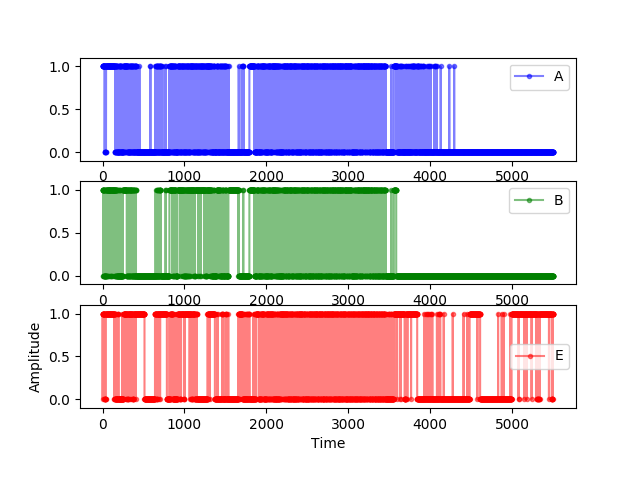
\includegraphics[width=0.65\textwidth ]
		{Bilder/a4-q0-2.png}
		\caption{\textit{quant0}}
		\label{fig:4.1}
\end{figure}


\begin{figure}[hbt!]
	\centering
		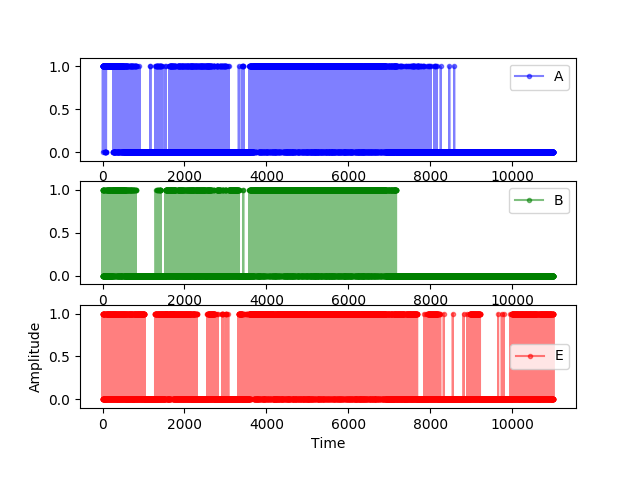
\includegraphics[width=0.65\textwidth ]
		{Bilder/a4-q1-2.png}
		\caption{\textit{quant1}}
		\label{fig:4.2}
\end{figure}


\begin{figure}[hbt!]
	\centering
		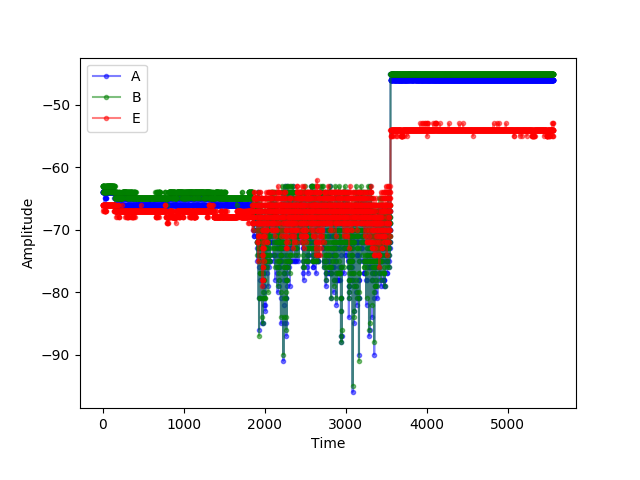
\includegraphics[width=0.65\textwidth ]
		{Bilder/a4-q0-1.png}
		\caption{\textit{Signalstärkenverlauf}}
		\label{fig:4.3}
\end{figure}

\begin{comment}
Wenn man Abbildung~\ref{fig:4.1} betrachtet, so erkennt man, 
dass Einflüsse wie Bewegung und Distanz eine große Rolle 
spielen.\\
Analysiert man die Unterschiede so wird klar, dass Bewegung
und größere Distanz einen Angreifer benachteiligen.	
\end{comment}

\newpage
Als nächstes wurde mit den Ausgaben dieses Befehls getestet.
\begin{python}
python konk_data.py -A 1_ohneBwg_A_B.csv 2_mBwg_A_B.csv -B 1_ohneBwg_B_A.csv 
2_mBwg_B_A.csv -E 1_ohneBwg_E_A.csv 2_mBwg_E_A.csv
\end{python}


\begin{figure}[hbt!]
	\centering
		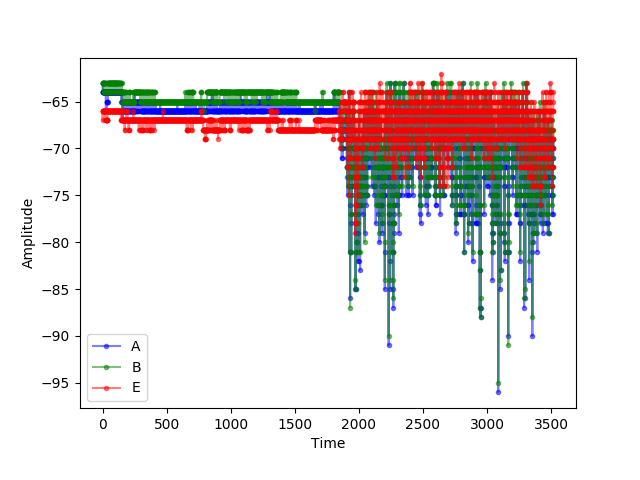
\includegraphics[width=0.65\textwidth ]
		{Bilder/a4-q0-1bis2.png}
		\caption{\textit{Signalstärkenverlauf}}
		\label{fig:4.4}
\end{figure}


\begin{figure}[hbt!]
	\centering
		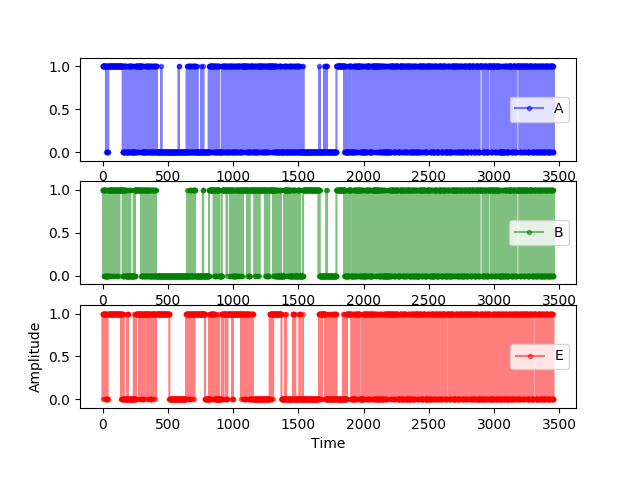
\includegraphics[width=0.65\textwidth ]
		{Bilder/a4-q0-1bis2-1.png}
		\caption{\textit{quant0}}
		\label{fig:4.5}
\end{figure}
\clearpage

\begin{figure}[hbt!]
	\centering
		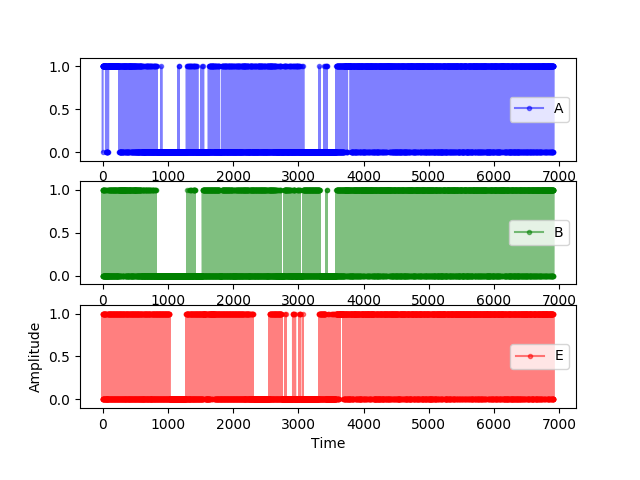
\includegraphics[width=0.65\textwidth ]
		{Bilder/a4-q1-1bis2-1.png}
		\caption{\textit{quant1}}
		\label{fig:4.6}
\end{figure}


Anschließend wurde mit den Ausgaben dieses Befehls getestet.
\begin{python}
python konk_data.py -A 3.a_mBwg_A_B.csv 3.a_ohneBwg_A_B.csv 3.b_mBwg_A_B.csv 
3.b_ohneBwg_A_B.csv  -B 3.a_mBwg_B_A.csv 3.a_ohneBwg_B_A.csv 3.b_mBwg_B_A.csv 
3.b_ohneBwg_B_A.csv -E 3.a_mBwg_E_A.csv 3.a_ohneBwg_E_A.csv 3.b_mBwg_E_A.csv 
3.b_ohneBwg_E_A.csv 
\end{python}

\begin{figure}[hbt!]
	\centering
		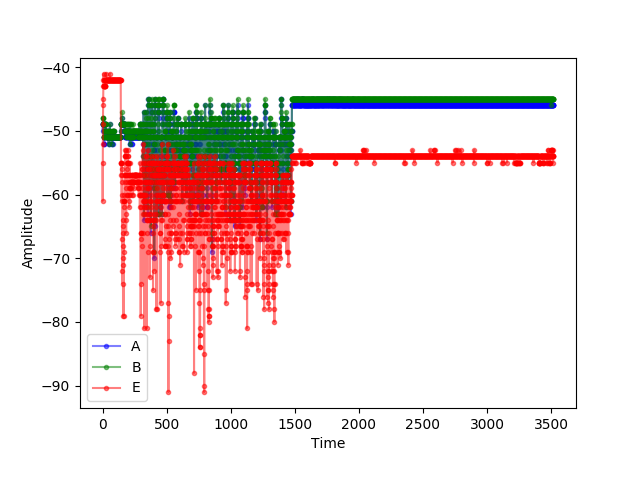
\includegraphics[width=0.65\textwidth ]
		{Bilder/a4-q0-3.png}
		\caption{\textit{Signalstärkenverlauf}}
		\label{fig:4.7}
\end{figure}


\begin{figure}[hbt!]
	\centering
		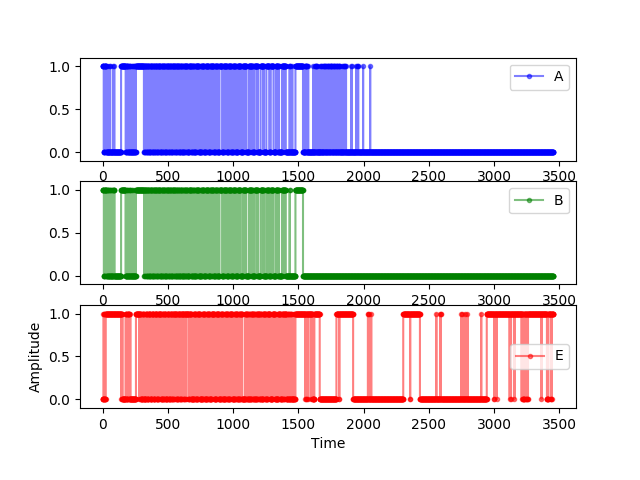
\includegraphics[width=0.65\textwidth ]
		{Bilder/a4-q0-3-1.png}
		\caption{\textit{quant0}}
		\label{fig:4.8}
\end{figure}


\begin{figure}[hbt!]
	\centering
		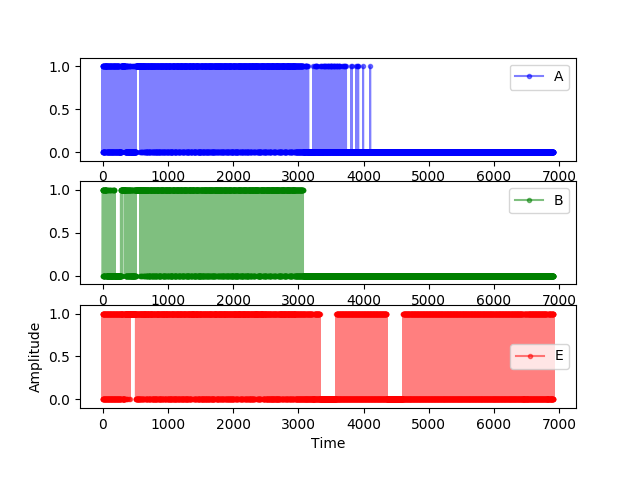
\includegraphics[width=0.65\textwidth ]
		{Bilder/a4-q1-3-1.png}
		\caption{\textit{quant1}}
		\label{fig:4.9}
\end{figure}



\glqq Gibt es einen Zusammenhang zwischen dem Verwendeten
Quantisierer und der Stärke des Angreifers?\grqq
Wie Abbildungen~\ref{fig:4.4} und ~\ref{fig:4.5} zeigen, 
bietet der  \textit{quant0}, also der 
\textit{mean quantizer} dem Angreifer einen leichten Vorteil,
zumindest, wenn die Bedingungen gut sind.
\glqq Welche Rolle spielt die Entfernung des Angreifers 
zu Alice/Bob\grqq
In Abbildungen~\ref{fig:4.8} und ~\ref{fig:4.9} ist klar zu 
erkennen, dass zunehmende Distanz einen Angreifer klar
benachteiligt.
\glqq Welche Rolle spielt die Bewegung im Raum?\grqq
Bewegung im Raum benachteiligt den Angreifer. Die 
Wirkung davon sieht man in Abbildungen~\ref{fig:4.4} 
und~\ref{fig:4.5}.


\subsection*{Repetition Attack}
Wie in der Vorlesung erwähnt wurde, ist es möglich
von einem Angreifer zyklische Bewegungen
auszunutzen, siehe Beispiel Modelleisenbahn.

\begin{figure}[hbt!]
	\centering
		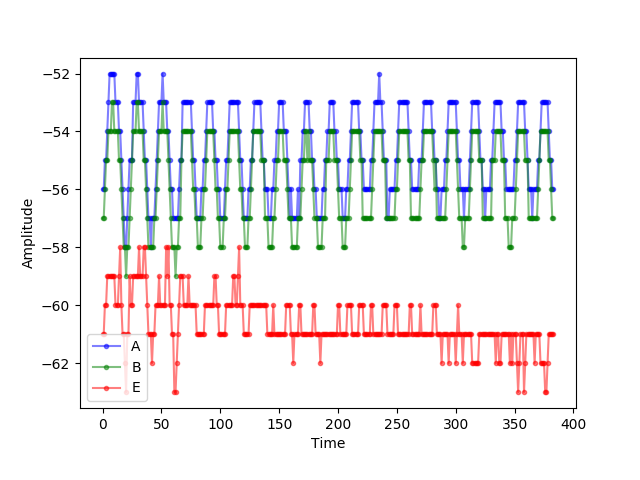
\includegraphics[width=0.65\textwidth ]
		{Bilder/a4-2.png}
		\caption{\textit{Signalstärkenverlauf}}
		\label{fig:4.10}
\end{figure}


\begin{figure}[hbt!]
	\centering
		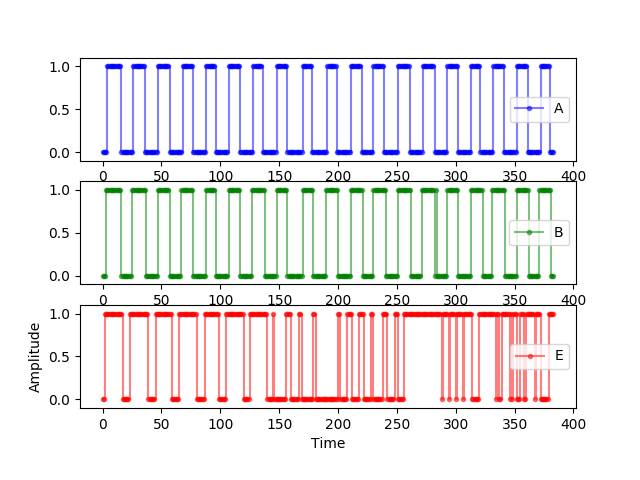
\includegraphics[width=0.65\textwidth ]
		{Bilder/a4-2-q0.png}
		\caption{\textit{quant0}}
		\label{fig:4.11}
\end{figure}


\begin{figure}[hbt!]
	\centering
		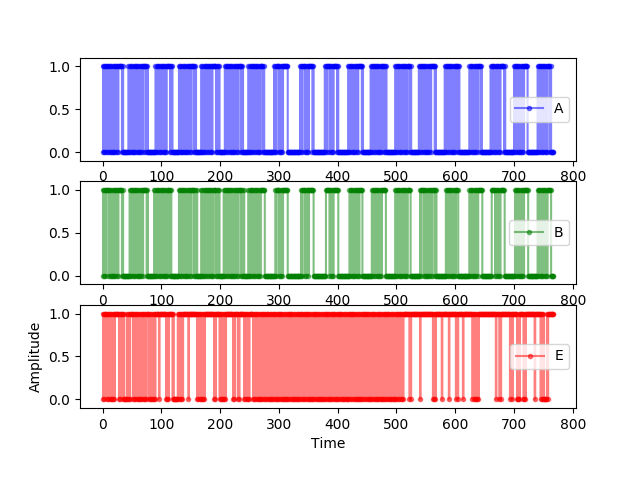
\includegraphics[width=0.65\textwidth ]
		{Bilder/a4-2-q1.png}
		\caption{\textit{quant1}}
		\label{fig:4.12}
\end{figure}


Es sind Muster zu erkennen, wobei 
Eves Muster eigentlich noch gleichmäßiger wäre,
aber die Messbedingungen waren nicht ideal.\\[3mm]
Es gibt erkennbare Unterschiede zwischen den
Quantisierern, wobei Eve \textit{quant0} bevorzugen
würde. Zyklische Bewegungen scheinen tatsächlich 
ausnutzbar zu sein für einen Angreifer. Eve muss dabei
unter anderem die Periode richtig schätzen.


\subsection*{Prediction Attack}

\begin{figure}[hbt!]
	\centering
		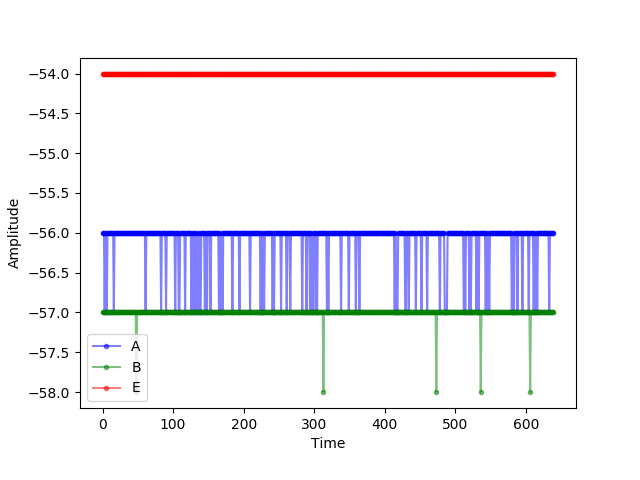
\includegraphics[width=0.65\textwidth ]
		{Bilder/a4-3.png}
		\caption{\textit{Signalstärkenverlauf}}
		\label{fig:4.13}
\end{figure}


\begin{figure}[hbt!]
	\centering
		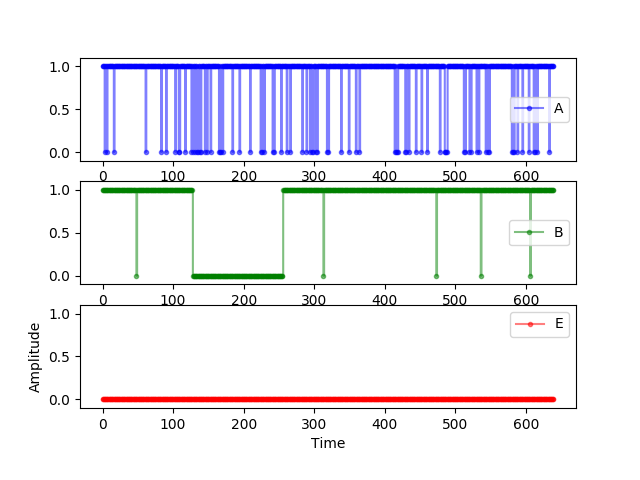
\includegraphics[width=0.65\textwidth ]
		{Bilder/a4-3-q0.png}
		\caption{\textit{quant0}}
		\label{fig:4.14}
\end{figure}


\begin{figure}[hbt!]
	\centering
		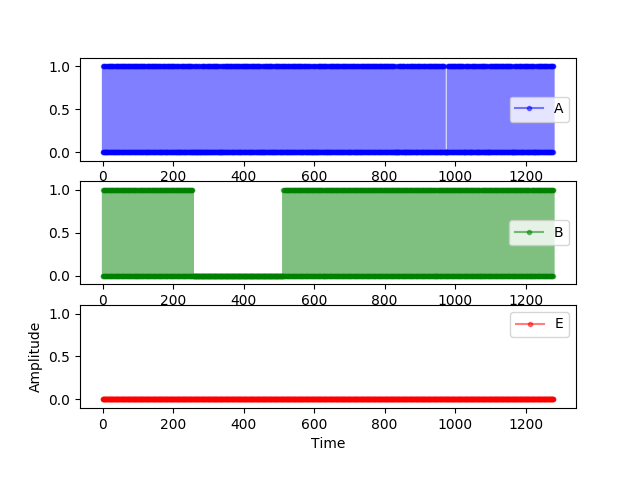
\includegraphics[width=0.65\textwidth ]
		{Bilder/a4-3-q1.png}
		\caption{\textit{quant1}}
		\label{fig:4.15}
\end{figure}

Betrachtet man Abbildungen~\ref{fig:4.14} und 
~\ref{fig:4.15}
kann man zum Entschluss kommen, dass Eve zumindest 
bei \textit{quant0} diese Attacke nutzen könnte um die 
Entropie zwischen Alice und Bob möglichst weit zu 
reduzieren. Alternativ könnte man diesen Angriff als 
\textit{denial-of-service-Attacke} nutzen um eine
erfolgreiche Schlüsseleinigung zwischen Alice und Bob 
zu torpedieren oder sogar zu verhindern. Hier ist
\textit{quant1} deutlich besser, im Sinne von, dass sich
die Quantiserung von Alice und Bob mehr ähneln.
\clearpage

\subsection*{Eigener Angriff}

Idee: Benutze Alufolie und Eisengusspfannen um zu sorgen, dass
Bob möglichst schwach empfängt.


\begin{figure}[hbt!]
	\centering
		\includegraphics[width=0.7\textwidth ]
		{Bilder/a4-4-foto1.jpg}
		\caption{\textit{Vielfach mit Alufolie umwickelt}}
		\label{fig:4.16}
\end{figure}	

\begin{figure}[hbt!]
	\centering
		\includegraphics[width=0.7\textwidth ]
		{Bilder/a4-4-foto2.jpg}
		\caption{\textit{Sakrophag aus Pfannen}}
		\label{fig:4.17}
\end{figure}	

\begin{figure}[hbt!]
	\centering
		\includegraphics[width=0.7\textwidth ]
		{Bilder/a4-4.png}
		\caption{\textit{Signalstärkenverlauf}}
		\label{fig:4.18}
\end{figure}

\begin{figure}[hbt!]
	\centering
		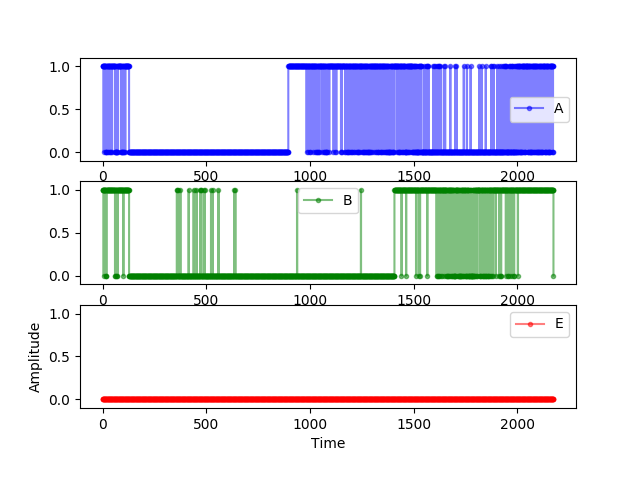
\includegraphics[width=0.7\textwidth ]
		{Bilder/a4-4-q0.png}
		\caption{\textit{quant0}}
		\label{fig:4.18}
\end{figure}
\clearpage


\begin{figure}[hbt!]
	\centering
		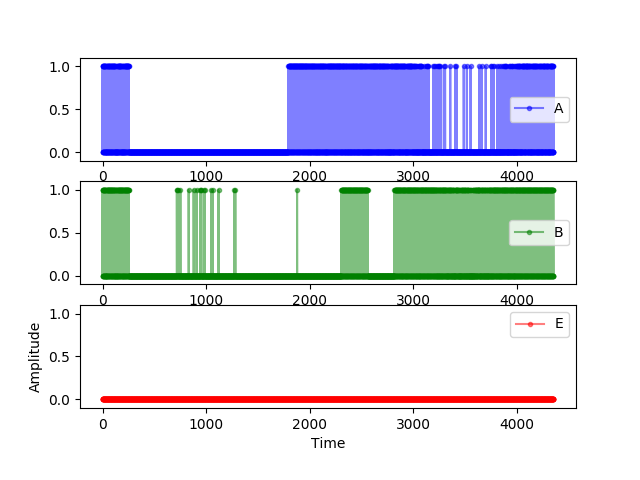
\includegraphics[width=0.7\textwidth ]
		{Bilder/a4-4-q1.png}
		\caption{\textit{quant1}}
		\label{fig:4.19}
\end{figure}

Möglichweise ist es machbar, wenn man diesen Angriff
noch etwas ausfeilt, dass am Ende nur noch Nullen 
quantisiert werden und somit die Schlüsselgenerierung 
manipuliert werden kann. Ansonsten ist es als
\textit{denial-of-service-Attacke} einsetzbar.
Wie zuvor auch, ist hier \textit{quant1} etwas 
besser.
\newpage
\section{Reading Assignment}

\subsection{Nennen Sie 5 verschiedene Quellen für Entropie}

\large
Physikalische Phänomene
\normalsize

\begin{itemize}
    \item Radioaktiver Zerfall
    \item Transmission von Photonen
    \item Thermisches Rauschen (Johnson-Nyquist-Rauschen)
    \item Geräusche der Atmosphäre
    \item Jitter
\end{itemize}


\large
Mensch-Gerät Interaktion
\normalsize

\begin{itemize}
    \item Dauer von Tastendrücken und andere Zeitmessungen
    \item Tasten-und Mausbewegungen
    \item Bewegungs- und Beschleunigungssensoren
\end{itemize}

\subsection{Wie viele Samples aus einem Smartphone Accelerator benötigen wir um einen 128 bit key zu
erstellen?}



\glqq Since the recommended security level for almost 
random bits is $\epsilon = 2^{-80}$. According to the 
heuristic (1) we need roughly 128/0.125  = 1024
samples to extract a 128-bit key. However taking into 
account the true error in our Theorem 1 we see that we 
need at least n ≈ 2214 bits!\grqq  \\~\\

Laut dem Paper, welches sie auf Theoreme stützt, 
braucht man mindestens 1024 Samples. Hinzu kommt 
allerdings, dass empfohlen wird, ein \textit{n} 
mit mehr als 2214 Bitlänge zu wählen.


\subsection{Wie groß ist der Unterschied an tatsächlich extrahierbarer Entropie und Shannon Entropie?}

\begin{figure}[hbt!]
	\centering
		
\includegraphics[width=1\textwidth ]
		{Bilder/a5-Corollary1.png}
		\caption{Auszug aus dem Paper}
		\label{fig:5.1}
\end{figure}
\clearpage

\glqq In information theory
most widely used is Shannon entropy, which quantifies 
the encoding length of a given distribution. In turn, 
cryptographers use the more conservative notion
called min-entropy, which quantifies unpredictability. 
In general, there is a large
gap between these two measures: the min-entropy of an 
n-bit string might be only
$O(1)$ whereas its Shannon entropy as big 
as $\Omega (n)$.\grqq \\    

Die min-Entropie eines n-bit langen stringes kann konstant
sein, wobei gleichzeitig seine Shannon Entropie linear oder
größer zu \textit{n} sein kann.\\\\

Von den 2214 bits können nur etwa 128 bits mit nahezu 
zufällig gleichverteilter Qualität extrahiert werden.
Das ist ein Verhältnis von $\frac{128}{2214} ≈ 0.0578$
oder anders gesagt: Der Schlüssel hat hier nur die Länge 
von 5,78\% von der Bitlänge des Samples.





\begin{comment}
% Beispiel für einen Hyperlink 	
\href{https://www.rub.de}{hier klicken}

% Beispiel für Bilder mit Caption und Referenz
\begin{figure}[hbt!]
	\centering
		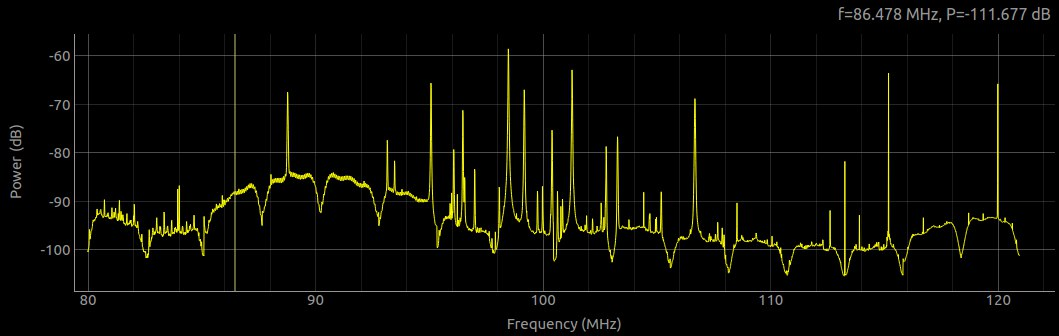
\includegraphics[width=1\textwidth ]
		{Bilder/a3_rtl_sdr.jpg}
		\caption{Hier Caption einfügen}
		\label{fig:Labelx}
\end{figure}

% Als Beispiel wie man referenziert
~\ref{fig:Labelx}

% Beispiel für das Einfügen von Python Code
\begin{python}
print("Hello World")
\end{python}

% Beispiel für das Erzwingen von Abstand (selbe Zeile)
\hspace{0.5mm}

% Beispiel für das Erzwingen von Abstand (nach unten)
\\[0.7cm]

%Beispiel für einen Pseudocode
\subsection*{b) Pseudocode}
\begin{algorithm}
\caption{Pseudocode}
\begin{algorithmic}[1]
\State $range = max[RSS] - min[RSS]$
\State $N \in [0, log_2 RSS]$
\State $M = 2^N$
\State $RSS[] \to M$ intervalls $I[]$ of equal size
\State Choose $N$ bit assignment $\forall$ $M$ intervalls
\For{$t \to len(RSS[])$}
\For{$i \to len(I[]$}
\If{$RSS[t] \in I[i]$}
\State $bitstream \gets$ bit assignment
\EndIf
\EndFor
\EndFor\\
\Return $bitstream$
\end{algorithmic}
\end{algorithm}

% Beispiel für ein Tabelle mit vergrößerter Schrift
\Large
\begin{tabular}{ |p{3cm}|||p{3cm}|p{3cm}||p{3cm}|p{3cm}|}
    \hline
    \multicolumn{5}{|c|}{Teilaufgabe 1: $A\rightarrow B$} \\
    \hline
    Blockgröße & Mittel Bob & Median Bob & Mittel Eve & Median Eve\\
    \hline
    \hspace{3.2mm}30 & 0.2290 & 0.1756 & 0.1798 & 0.1428\\
    100 & 0.2219 & 0.1848 & 0.1341 & 0.1053\\
    200 & 0.2401 & 0.2377 & 0.0946 & 0.0748\\
    250 & 0.2591 & 0.2328 & 0.1495 & 0.1260\\
    300 & 0.2791 & 0.2108 & 0.1784 & 0.1130\\
    \hline
\end{tabular}
\normalsize

% Öffnende und schließende deutsche Anführungszeichen
\glqq Zitierter Text komm hierhin \grqq  



\end{comment}

\end{document}